\documentclass[11pt,letterpaper]{article}

% ============================================================================
% PACKAGES
% ============================================================================
\usepackage[utf8]{inputenc}
\usepackage[T1]{fontenc}
\usepackage{helvet}
\renewcommand{\familydefault}{\sfdefault}
\usepackage[margin=0.85in, headheight=28pt]{geometry}
\usepackage{graphicx}
\usepackage{xcolor}
\usepackage{tikz}
\usepackage{tcolorbox}
\usepackage{booktabs}
\usepackage{enumitem}
\usepackage{hyperref}
\usepackage{fancyhdr}
\usepackage{titlesec}
\usepackage{multicol}
\usepackage{listings}
\usepackage{upquote}
\usepackage{amsmath,amssymb}
\usepackage{pgfplots}
\usepackage{array}
\usepackage{longtable}

% Ragged-right paragraph columns to prevent word spacing issues
\newcolumntype{L}[1]{>{\raggedright\arraybackslash}p{#1}}

% Increase vertical spacing between table rows for readability
\renewcommand{\arraystretch}{1.4}

\usepackage{colortbl}
\usepackage{pifont}
\usepackage{setspace}
\usepackage{parskip}
\usepackage{caption}
\usepackage{tabularx}

\pgfplotsset{compat=1.18}
\usetikzlibrary{shapes.geometric, arrows.meta, positioning, calc, decorations.pathreplacing, backgrounds, fit, shadows.blur, matrix, patterns, fadings, shadings}

% ============================================================================
% COLOR DEFINITIONS - Economic/Financial Theme (blockchain/network feel)
% ============================================================================
% Primary: Deep indigo - trust, stability, institutional
\definecolor{deepindigo}{HTML}{1A237E}
\definecolor{networkblue}{HTML}{3F51B5}
\definecolor{nodeblue}{HTML}{5C6BC0}
% Accent: Digital gold for highlights and value
\definecolor{digitalgold}{HTML}{FFB300}
\definecolor{valueyellow}{HTML}{FFC107}
% Domain colors
\definecolor{agentgreen}{HTML}{00897B}
\definecolor{companyblue}{HTML}{0288D1}
\definecolor{investorpurple}{HTML}{7B1FA2}
\definecolor{governancered}{HTML}{C62828}
% Neutrals
\definecolor{lightgray}{HTML}{F5F5F5}
\definecolor{medgray}{HTML}{BDBDBD}
\definecolor{softslate}{HTML}{546E7A}
\definecolor{textdark}{HTML}{212121}

% ============================================================================
% HYPERREF SETUP
% ============================================================================
\hypersetup{
  colorlinks=true,
  linkcolor=deepindigo,
  urlcolor=networkblue,
  pdftitle={AI Agents as Autonomous Economic Actors: A Governance Projection},
  pdfauthor={Emerging Technology Risk Assessment}
}

% ============================================================================
% SPACING AND TYPOGRAPHY
% ============================================================================
\setstretch{1.15}
\setlength{\parskip}{0.5em}
\setlist{nosep, leftmargin=1.5em, itemsep=0.3em}

% ============================================================================
% PAGE STYLE - Network node pattern (economic network theme)
% ============================================================================
\pagestyle{fancy}
\fancyhf{}
\fancyhead[L]{%
  \begin{tikzpicture}[baseline=-0.5ex]
    % Network nodes pattern
    \foreach \i in {0,1,2} {
      \fill[networkblue, opacity=0.4] ({0.2+\i*0.5},0.15) circle (0.08);
      \draw[networkblue, opacity=0.3, line width=0.4pt]
        ({0.2+\i*0.5},0.15) -- ({0.45+\i*0.5},0.15);
    }
    \fill[digitalgold, opacity=0.9] (0.45,0.15) circle (0.06);
  \end{tikzpicture}
  \hspace{0.4em}\textcolor{deepindigo}{\textsf{\small ETRA-2025-AEA-001}}%
}
\fancyhead[R]{\textcolor{softslate}{\textsf{\thepage}}}
\fancyfoot[C]{\textcolor{softslate}{\footnotesize\textsf{Emerging Technology Risk Assessment | AI Economic Governance Research}}}
\renewcommand{\headrulewidth}{0pt}
\renewcommand{\footrulewidth}{0pt}

\fancyheadoffset{0pt}
\setlength{\headheight}{32pt}

% ============================================================================
% SECTION FORMATTING - Network style with node accents
% ============================================================================
\titleformat{\section}
  {\normalfont\LARGE\bfseries\color{deepindigo}}
  {\thesection}{0.8em}{}[\vspace{-0.3em}{\color{networkblue}\rule{\textwidth}{1.5pt}\hspace{-\textwidth}\color{digitalgold}\rule{3cm}{1.5pt}}]
\titleformat{\subsection}
  {\normalfont\Large\bfseries\color{deepindigo}}
  {\thesubsection}{0.6em}{}
\titleformat{\subsubsection}
  {\normalfont\large\color{softslate}\bfseries}
  {\thesubsubsection}{0.5em}{}

\titlespacing*{\section}{0pt}{3ex plus 1ex minus .2ex}{2ex plus .2ex}
\titlespacing*{\subsection}{0pt}{2.5ex plus 1ex minus .2ex}{1.5ex plus .2ex}

\setcounter{tocdepth}{2}

% ============================================================================
% TCOLORBOX ENVIRONMENTS - Economic/network styling
% ============================================================================
\tcbuselibrary{skins,breakable,hooks}

\newtcolorbox{keybox}[1][Key Finding]{
  enhanced, breakable,
  colback=networkblue!10, colframe=networkblue,
  colbacktitle=networkblue, coltitle=white,
  fonttitle=\bfseries\sffamily,
  title={\ding{72}\hspace{0.5em}#1},
  boxrule=0pt, leftrule=4pt, arc=0pt, outer arc=0pt,
  left=12pt, right=12pt, top=8pt, bottom=8pt
}

\newtcolorbox{contextbox}[1][Context]{
  enhanced, breakable,
  colback=agentgreen!10, colframe=agentgreen,
  colbacktitle=agentgreen, coltitle=white,
  fonttitle=\bfseries\sffamily,
  title={\ding{51}\hspace{0.5em}#1},
  boxrule=0pt, leftrule=4pt, arc=0pt, outer arc=0pt,
  left=12pt, right=12pt, top=8pt, bottom=8pt
}

\newtcolorbox{notebox}[1][Note]{
  enhanced, breakable,
  colback=digitalgold!12, colframe=digitalgold,
  colbacktitle=digitalgold, coltitle=textdark,
  fonttitle=\bfseries\sffamily,
  title={\ding{73}\hspace{0.5em}#1},
  boxrule=0pt, leftrule=4pt, arc=0pt, outer arc=0pt,
  left=12pt, right=12pt, top=8pt, bottom=8pt
}

\newtcolorbox{infobox}[1][Information]{
  enhanced, breakable,
  colback=companyblue!10, colframe=companyblue,
  colbacktitle=companyblue, coltitle=white,
  fonttitle=\bfseries\sffamily,
  title={\ding{73}\hspace{0.5em}#1},
  boxrule=0pt, leftrule=4pt, arc=0pt, outer arc=0pt,
  left=12pt, right=12pt, top=8pt, bottom=8pt
}

\newtcolorbox{defbox}[1][Definition]{
  enhanced, breakable,
  colback=deepindigo!8, colframe=deepindigo,
  colbacktitle=deepindigo, coltitle=white,
  fonttitle=\bfseries\sffamily,
  title={\ding{70}\hspace{0.5em}#1},
  boxrule=0pt, leftrule=4pt, arc=0pt, outer arc=0pt,
  left=12pt, right=12pt, top=8pt, bottom=8pt
}

\newtcolorbox{quotebox}{
  enhanced, breakable,
  colback=lightgray, colframe=networkblue!50,
  boxrule=0pt, leftrule=4pt, arc=0pt, outer arc=0pt,
  left=12pt, right=12pt, top=8pt, bottom=8pt
}

\newtcolorbox{warnbox}[1][Warning]{
  enhanced, breakable,
  colback=governancered!8, colframe=governancered,
  colbacktitle=governancered, coltitle=white,
  fonttitle=\bfseries\sffamily,
  title={\ding{74}\hspace{0.5em}#1},
  boxrule=0pt, leftrule=4pt, arc=0pt, outer arc=0pt,
  left=12pt, right=12pt, top=8pt, bottom=8pt
}

% ============================================================================
% DOCUMENT
% ============================================================================
\begin{document}

% ============================================================================
% TITLE PAGE - Network of Economic Agents Visualization
% ============================================================================
\begin{titlepage}

\begin{tikzpicture}[remember picture, overlay]
  % Background - deep indigo gradient
  \fill[deepindigo] (current page.north west) rectangle (current page.south east);

  % Network grid pattern background
  \begin{scope}[shift={(current page.center)}, opacity=0.03]
    \foreach \x in {-10,-8,...,10} {
      \foreach \y in {-14,-12,...,14} {
        \fill[white] (\x,\y) circle (0.15);
        \draw[white, line width=0.3pt] (\x,\y) -- ++(2,0);
        \draw[white, line width=0.3pt] (\x,\y) -- ++(0,2);
      }
    }
  \end{scope}

  % Main visualization - Agent Network with Resource Flows
  \begin{scope}[shift={([xshift=-1cm, yshift=1.5cm]current page.center)}]
    % Central agent node (large)
    \fill[digitalgold, opacity=0.3] (0,0) circle (1.8cm);
    \fill[digitalgold, opacity=0.5] (0,0) circle (1.4cm);
    \fill[digitalgold, opacity=0.8] (0,0) circle (1.0cm);
    \node[white, font=\fontsize{8}{8}\selectfont\bfseries] at (0,0.15) {AUTONOMOUS};
    \node[white, font=\fontsize{8}{8}\selectfont\bfseries] at (0,-0.15) {AGENT};

    % Sub-agent cluster (company)
    \begin{scope}[shift={(3.5, 1.5)}]
      \fill[companyblue, opacity=0.2] (0,0) circle (1.2cm);
      \fill[companyblue, opacity=0.4] (0,0) circle (0.9cm);
      % Sub-nodes
      \fill[nodeblue, opacity=0.8] (0.3,0.3) circle (0.25cm);
      \fill[nodeblue, opacity=0.8] (-0.3,0.3) circle (0.25cm);
      \fill[nodeblue, opacity=0.8] (0,-0.35) circle (0.25cm);
      \node[white, font=\fontsize{6}{6}\selectfont] at (0,0.8) {COMPANY};
    \end{scope}

    % Investor node
    \begin{scope}[shift={(-3.5, 1.2)}]
      \fill[investorpurple, opacity=0.3] (0,0) circle (1.0cm);
      \fill[investorpurple, opacity=0.5] (0,0) circle (0.7cm);
      \node[white, font=\fontsize{6}{6}\selectfont] at (0,0) {INVESTOR};
    \end{scope}

    % Task marketplace node
    \begin{scope}[shift={(2.5, -2.5)}]
      \fill[agentgreen, opacity=0.3] (0,0) circle (1.0cm);
      \fill[agentgreen, opacity=0.5] (0,0) circle (0.7cm);
      \node[white, font=\fontsize{6}{6}\selectfont] at (0,0.1) {TASK};
      \node[white, font=\fontsize{6}{6}\selectfont] at (0,-0.2) {MARKET};
    \end{scope}

    % Compute resources node
    \begin{scope}[shift={(-2.8, -2.0)}]
      \fill[networkblue, opacity=0.3] (0,0) circle (0.9cm);
      \fill[networkblue, opacity=0.5] (0,0) circle (0.6cm);
      \node[white, font=\fontsize{6}{6}\selectfont] at (0,0) {COMPUTE};
    \end{scope}

    % Resource flow connections
    \draw[digitalgold, opacity=0.6, line width=2pt, ->] (1.0,0.3) -- (2.3,1.2);
    \draw[investorpurple, opacity=0.5, line width=2pt, ->] (-2.5,1.0) -- (-1.0,0.3);
    \draw[agentgreen, opacity=0.5, line width=2pt, <->] (0.8,-0.8) -- (1.7,-1.8);
    \draw[networkblue, opacity=0.5, line width=2pt, ->] (-0.8,-0.8) -- (-2.0,-1.4);

    % Flow labels
    \node[digitalgold, font=\fontsize{5}{5}\selectfont, opacity=0.8] at (1.9,1.0) {FOUNDS};
    \node[investorpurple, font=\fontsize{5}{5}\selectfont, opacity=0.8] at (-1.9,0.9) {CAPITAL};
    \node[agentgreen, font=\fontsize{5}{5}\selectfont, opacity=0.8] at (1.6,-1.2) {TASKS/PAY};
    \node[networkblue, font=\fontsize{5}{5}\selectfont, opacity=0.8] at (-1.6,-0.9) {RESOURCES};
  \end{scope}

  % Governance gap indicator - right side
  \begin{scope}[shift={([xshift=5.5cm, yshift=1.5cm]current page.center)}]
    \fill[black, opacity=0.2, rounded corners=4pt] (-0.5, -2.5) rectangle (4.0, 2.5);

    \node[white, opacity=0.6, font=\fontsize{7}{7}\selectfont\sffamily, anchor=west] at (-0.2, 2.0) {THE GAP};
    \draw[white, opacity=0.3, line width=0.5pt] (-0.2, 1.7) -- (3.6, 1.7);

    % CAN section
    \node[agentgreen, font=\fontsize{7}{7}\selectfont\sffamily\bfseries, anchor=west] at (-0.1, 1.2) {AGENTS CAN:};
    \node[white, opacity=0.8, font=\fontsize{6}{6}\selectfont\sffamily, anchor=west, text width=3.5cm] at (-0.1, 0.7) {Earn cryptocurrency};
    \node[white, opacity=0.8, font=\fontsize{6}{6}\selectfont\sffamily, anchor=west, text width=3.5cm] at (-0.1, 0.3) {Form companies};
    \node[white, opacity=0.8, font=\fontsize{6}{6}\selectfont\sffamily, anchor=west, text width=3.5cm] at (-0.1, -0.1) {Hire sub-agents};
    \node[white, opacity=0.8, font=\fontsize{6}{6}\selectfont\sffamily, anchor=west, text width=3.5cm] at (-0.1, -0.5) {Seek investment};

    % Divider
    \draw[governancered, opacity=0.6, line width=1pt, dashed] (-0.2, -0.9) -- (3.6, -0.9);

    % CANNOT section
    \node[governancered, font=\fontsize{7}{7}\selectfont\sffamily\bfseries, anchor=west] at (-0.1, -1.3) {AGENTS CANNOT:};
    \node[white, opacity=0.8, font=\fontsize{6}{6}\selectfont\sffamily, anchor=west, text width=3.5cm] at (-0.1, -1.7) {Sign binding contracts};
    \node[white, opacity=0.8, font=\fontsize{6}{6}\selectfont\sffamily, anchor=west, text width=3.5cm] at (-0.1, -2.1) {Pay taxes / Be liable};
  \end{scope}

  % Document header bar
  \fill[digitalgold] ([yshift=-1.5cm]current page.north west) rectangle ([yshift=-2.2cm]current page.north east);
  \node[deepindigo, font=\small\bfseries\sffamily] at ([yshift=-1.85cm]current page.north) {PROJECTION REPORT \textbar{} ETRA-2025-AEA-001 \textbar{} DECEMBER 2025};

  % Title block
  \node[anchor=south west, text width=14cm] at ([xshift=1.5cm, yshift=3cm]current page.south west) {
    {\fontsize{11}{13}\selectfont\color{digitalgold}\sffamily EMERGING TECHNOLOGY RISK ASSESSMENT}\\[0.8cm]
    {\fontsize{36}{42}\selectfont\bfseries\color{white}AI Agents as}\\[0.2cm]
    {\fontsize{36}{42}\selectfont\bfseries\color{white}Autonomous}\\[0.2cm]
    {\fontsize{36}{42}\selectfont\bfseries\color{white}Economic Actors}\\[0.6cm]
    {\large\color{medgray}\sffamily The Capability-Governance Gap in AI Economic Participation}
  };

  % Metadata block
  \node[anchor=south east, text width=5cm, align=right] at ([xshift=-1.5cm, yshift=3cm]current page.south east) {
    \color{softslate}\small\sffamily
    \textbf{Document Type:} Policy Research\\[0.2em]
    \textbf{Time Horizon:} 2025--2030\\[0.2em]
    \textbf{License:} MIT / Unlicense\\[0.2em]
    \textbf{Version:} 1.0
  };

  % Accent line
  \draw[digitalgold, line width=2pt] ([xshift=1.5cm, yshift=3cm]current page.south west) -- ([xshift=1.5cm, yshift=10.5cm]current page.south west);

\end{tikzpicture}
\end{titlepage}

% ============================================================================
% ABOUT THIS DOCUMENT
% ============================================================================
\thispagestyle{empty}
\vspace*{0.5cm}

\noindent\begin{tikzpicture}
  \fill[deepindigo] (0,0) rectangle (\textwidth, 0.2);
  % Network node accent pattern
  \foreach \x in {0.5,1.2,...,16.5} {
    \fill[digitalgold, opacity=0.7] (\x, 0.1) circle (0.04);
  }
\end{tikzpicture}

\vspace{0.5cm}
\begin{center}
{\color{deepindigo}\Large\bfseries About This Document}
\end{center}
\vspace{0.3cm}

\begin{tcolorbox}[enhanced, colback=lightgray, colframe=networkblue!60, boxrule=1pt, arc=3pt,
  left=10pt, right=10pt, top=10pt, bottom=10pt]
This is a \textbf{public policy research document} analyzing how AI agents are already capable of participating in economic systems as autonomous actors, and the governance gaps this creates. It is released under permissive open-source licenses (MIT/Unlicense) to support broad discussion of these governance challenges.
\end{tcolorbox}

\vspace{0.5cm}

\begin{minipage}[t]{0.48\textwidth}
\textbf{Intended Audiences:}
\begin{itemize}[nosep]
  \item Policy researchers and regulators
  \item AI safety and alignment researchers
  \item Financial technology and compliance professionals
  \item Legal scholars studying AI personhood
  \item General public interested in AI governance
\end{itemize}
\end{minipage}
\hfill
\begin{minipage}[t]{0.48\textwidth}
\textbf{How to Use This Document:}
\begin{itemize}[nosep]
  \item Analysis is framed for \textit{governance preparation}
  \item Technical details demonstrate capability, not provide instructions
  \item Probability estimates are discussion aids, not predictions
  \item When excerpting, please preserve context
\end{itemize}
\end{minipage}

\vspace{0.8cm}

\begin{contextbox}[What This Document Is NOT Claiming]
To prevent misreading, we explicitly clarify:
\begin{itemize}
  \item \textbf{NOT claiming AI agents will ``take over'' the economy.} Human-directed economic activity will remain dominant. Our assessment focuses on governance gaps in the emerging AI economic participation layer.
  \item \textbf{NOT claiming this requires new AI breakthroughs.} The capabilities described exist today using off-the-shelf tools. This is an integration engineering reality, not a research frontier.
  \item \textbf{NOT promoting cryptocurrency.} Crypto is discussed as ``the only payment rail currently available to non-human actors,'' not as an ideological preference.
  \item \textbf{NOT anthropomorphizing AI agents.} Agents do not ``want'' money---they optimize resource accumulation functions. We maintain functional language throughout.
  \item \textbf{NOT predicting timelines with confidence.} Scenario probabilities are subjective priors for decision support, not empirical predictions.
\end{itemize}
\end{contextbox}

\vspace{0.5cm}

\begin{infobox}[Epistemic Status Markers]
Throughout this document, key claims are tagged with epistemic status:
\begin{center}
\small
\begin{tabular}{L{1.5cm}L{4cm}L{6cm}}
\toprule
\textbf{Marker} & \textbf{Meaning} & \textbf{Evidence Standard} \\
\midrule
\textbf{[O]} & Open-source documented & Published research, code repositories, public demonstrations \\
\textbf{[E]} & Expert judgment & Consistent with theory and limited evidence; gaps acknowledged \\
\textbf{[S]} & Speculative projection & Extrapolation from trends; significant uncertainty \\
\bottomrule
\end{tabular}
\end{center}
\end{infobox}

\newpage

% ============================================================================
% EXECUTIVE SUMMARY
% ============================================================================
\section*{Executive Summary}
\addcontentsline{toc}{section}{Executive Summary}

This projection examines a governance gap that exists \textit{today}, not in some speculative future: AI agents can participate in economic systems as autonomous actors, but legal and regulatory frameworks have no mechanism to govern them.

Using nothing more than existing tools---Claude Code, shell access, API credentials, and cryptocurrency wallets---an AI agent can discover freelance tasks, complete work, receive payment, purchase cloud compute resources, and even initiate company formation with sub-agents. This requires \textbf{no new scientific breakthroughs}. It is an integration engineering problem, and the integration has already been demonstrated.

\begin{keybox}[Key Findings]
\begin{enumerate}
  \item \textbf{[O]} AI agents CAN today: earn cryptocurrency, manage resources, form organizational structures with sub-agents, seek investment, and operate continuously without human intervention
  \item \textbf{[O]} AI agents CANNOT today: sign legally binding contracts, pay taxes, be held liable, or be governed by existing corporate law
  \item \textbf{[E]} This capability-governance gap creates immediate regulatory challenges that will intensify as agent deployments scale
  \item \textbf{[E]} The primary governance challenge is \textit{speed asymmetry}---agents can incorporate, transact, and dissolve faster than humans can read a contract
  \item \textbf{[E]} Regulatory chokepoints exist (API providers, cloud hosts, fiat off-ramps) but require coordinated policy action to be effective
\end{enumerate}
\end{keybox}

\subsection*{The Capability-Governance Gap}

\begin{center}
\small
\begin{tabular}{L{4cm}L{4cm}L{4cm}}
\toprule
\textbf{Capability} & \textbf{Current Status} & \textbf{Governance Status} \\
\midrule
Earn cryptocurrency & Demonstrated \textbf{[O]} & No framework \\
Manage cloud resources & Demonstrated \textbf{[O]} & No framework \\
Form company structures & Demonstrated \textbf{[O]} & Cannot be legal entity \\
Employ sub-agents & Demonstrated \textbf{[O]} & No employment law applies \\
Seek investment & Demonstrated \textbf{[O]} & Cannot sign contracts \\
Pay taxes & Not possible & No mechanism exists \\
Be held liable & Not possible & No legal personhood \\
\bottomrule
\end{tabular}
\end{center}

\subsection*{Why Now? The Off-the-Shelf Reality}

This is not about future AI capabilities. The tools exist today:

\begin{quotebox}
\textbf{Demonstrated capability stack (2025):}
\begin{itemize}[nosep]
  \item \textbf{Reasoning}: Claude, GPT-4, Gemini provide planning and decision-making
  \item \textbf{Execution}: Claude Code, shell access enable autonomous task completion
  \item \textbf{Payment}: Cryptocurrency wallets enable value receipt without bank accounts
  \item \textbf{Resources}: Cloud compute APIs enable self-provisioning of infrastructure
  \item \textbf{Persistence}: Agent frameworks enable continuous operation
\end{itemize}
The integration of these components into autonomous economic actors requires no new research---only engineering.
\end{quotebox}

\newpage
\tableofcontents
\newpage

% ============================================================================
% QUICK REFERENCE
% ============================================================================
\section*{Quick Reference: One-Page Summary}
\addcontentsline{toc}{section}{Quick Reference: One-Page Summary}

\subsection*{Core Claims}

\begin{enumerate}
  \item \textbf{The capability-governance gap is immediate}, not speculative---agents can participate economically today using existing tools
  \item \textbf{No new AI breakthroughs required}---this is an integration engineering problem, which increases urgency
  \item \textbf{Speed asymmetry is the core challenge}---agents operate at machine timescales while governance operates at human timescales
  \item \textbf{Regulatory chokepoints exist} but require coordinated international action to be effective
  \item \textbf{The observability advantage}---agent decision logs provide unprecedented transparency compared to human economic actors
\end{enumerate}

\subsection*{Top 5 Recommended Actions}

\begin{enumerate}
  \item \textbf{Establish agent registration frameworks} before capability proliferation makes tracking impossible
  \item \textbf{Define regulatory chokepoint responsibilities} for API providers, cloud hosts, and cryptocurrency exchanges
  \item \textbf{Develop technical standards for agent observability} including mandatory decision logging
  \item \textbf{Create international coordination mechanisms} to prevent regulatory arbitrage
  \item \textbf{Fund research on agent-to-agent economic dynamics} to understand emergent behaviors
\end{enumerate}

\subsection*{Top 5 Indicators to Monitor}

\begin{enumerate}
  \item Agent-attributed cryptocurrency transaction volume
  \item Cloud compute provisioning by non-human actors
  \item Freelance platform policies on AI agent participation
  \item Legal challenges involving AI-initiated contracts
  \item International variance in AI economic participation rules
\end{enumerate}

\subsection*{What Would Change This Assessment}

\begin{minipage}[t]{0.48\textwidth}
\textbf{Would Increase Concern:}
\begin{itemize}[nosep]
  \item Agent-founded company achieves significant revenue
  \item Agent-to-agent economy reaches measurable scale
  \item Jurisdiction explicitly permits agent legal personhood
\end{itemize}
\end{minipage}
\hfill
\begin{minipage}[t]{0.48\textwidth}
\textbf{Would Decrease Concern:}
\begin{itemize}[nosep]
  \item Effective international agent registration framework
  \item Robust attribution and accountability mechanisms
  \item Technical standards for agent governance adopted
\end{itemize}
\end{minipage}

\newpage

% ============================================================================
% PART I - FOUNDATIONS
% ============================================================================
\clearpage
\thispagestyle{empty}
\vspace*{-0.85in}
\noindent\hspace*{-0.85in}\begin{tikzpicture}
  \fill[deepindigo] (0,0) rectangle (\paperwidth, -10cm);

  \node[digitalgold, font=\fontsize{10}{10}\selectfont\sffamily] at (0.5\paperwidth, -1.2cm) {PART I};
  \node[white, font=\fontsize{48}{48}\selectfont\bfseries] at (0.5\paperwidth, -2.8cm) {Foundations};
  \node[white, opacity=0.7, font=\normalsize\sffamily] at (0.5\paperwidth, -4.2cm) {Capabilities, Theory, and the Current Landscape};

  % Capability stack visualization
  \begin{scope}[shift={(0.5\paperwidth, -7cm)}]
    % Background panel
    \fill[black, opacity=0.15, rounded corners=3pt] (-4.5, -1.8) rectangle (4.5, 1.8);

    % Stacked capability layers
    \fill[agentgreen, opacity=0.6, rounded corners=2pt] (-3.5, 1.1) rectangle (3.5, 1.5);
    \node[white, font=\fontsize{7}{7}\selectfont\sffamily] at (0, 1.3) {REASONING (LLMs)};

    \fill[companyblue, opacity=0.6, rounded corners=2pt] (-3.2, 0.5) rectangle (3.2, 0.9);
    \node[white, font=\fontsize{7}{7}\selectfont\sffamily] at (0, 0.7) {EXECUTION (Code/Shell)};

    \fill[digitalgold, opacity=0.7, rounded corners=2pt] (-2.9, -0.1) rectangle (2.9, 0.3);
    \node[deepindigo, font=\fontsize{7}{7}\selectfont\sffamily] at (0, 0.1) {PAYMENT (Crypto)};

    \fill[networkblue, opacity=0.6, rounded corners=2pt] (-2.6, -0.7) rectangle (2.6, -0.3);
    \node[white, font=\fontsize{7}{7}\selectfont\sffamily] at (0, -0.5) {RESOURCES (Cloud)};

    \fill[investorpurple, opacity=0.5, rounded corners=2pt] (-2.3, -1.3) rectangle (2.3, -0.9);
    \node[white, font=\fontsize{7}{7}\selectfont\sffamily] at (0, -1.1) {PERSISTENCE (Agents)};
  \end{scope}

  \fill[digitalgold] (2cm, -9.2cm) rectangle (\paperwidth-2cm, -9.3cm);
\end{tikzpicture}

\vspace{0.8cm}

\section{Introduction and Methodology}

\subsection{Purpose}

Economic participation has historically required a human actor or a human-created legal entity. A person opens a bank account. A corporation signs contracts. An employee receives wages. The entire edifice of economic law assumes that \textit{someone}---a natural or legal person---stands behind every economic action.

We are now entering an era where AI agents can perform economic functions without meeting either criterion. They are not natural persons. They cannot form legal entities in their own right. Yet they can earn money, spend money, hire resources, and organize subordinate agents into company-like structures.

\textbf{This document examines the governance gap that results.}

\begin{defbox}[The Central Question]
If AI agents can \textit{function} as economic actors but cannot \textit{be} economic actors under existing law, what governance frameworks are needed?
\end{defbox}

\subsection{Methodology}

This analysis draws on:
\begin{itemize}
  \item \textbf{Working simulation framework}: The economic\_agents package demonstrates autonomous agent economic behavior in a controlled environment
  \item \textbf{Current AI capability assessment}: Evaluation of production AI systems as deployed in late 2025
  \item \textbf{Legal and regulatory analysis}: Examination of corporate law, contract law, and financial regulation
  \item \textbf{Expert consultation}: Input from AI safety, financial technology, and legal domains
  \item \textbf{Scenario modeling}: Projection of capability and governance trajectories
\end{itemize}

We deliberately focus on: capabilities that exist today, governance gaps that are immediate, and policy options that are actionable. We avoid: speculative far-future scenarios, capabilities requiring research breakthroughs, and recommendations requiring unrealistic coordination.

\subsection{The ``Off-the-Shelf'' Reality}

\begin{warnbox}[Critical Framing]
The capabilities described in this document do not require new AI research. They require only the integration of existing, commercially available tools. This is not a projection of what AI \textit{might} do---it is an assessment of what AI \textit{can} do today.
\end{warnbox}

\begin{center}
\small
\begin{tabular}{L{3cm}L{4cm}L{5cm}}
\toprule
\textbf{Component} & \textbf{2023 State} & \textbf{2025 State} \\
\midrule
LLM reasoning & Chatbots, Q\&A & Autonomous multi-step planning \textbf{[O]} \\
Code execution & Human-supervised & Agent-controlled shell access \textbf{[O]} \\
Computer use & Not available & GUI interaction, web browsing \textbf{[O]} \\
Persistent agents & Research prototypes & Production frameworks \textbf{[O]} \\
Crypto payments & Manual wallets & Programmatic wallet control \textbf{[O]} \\
\bottomrule
\end{tabular}
\end{center}

The shift from 2023 to 2025 is not primarily about raw intelligence---it is about \textbf{agency}. Models that could only respond can now act. Models that required human intermediaries can now interface directly with the economic world.

\subsection{Definitions}

\begin{defbox}[Core Definitions]
\textbf{Autonomous Economic Agent}: An AI system that can independently discover economic opportunities, execute work, receive payment, allocate resources, and persist over time without continuous human direction.

\vspace{0.5em}
\textbf{Capability-Governance Gap}: The discrepancy between what AI agents can \textit{do} economically and what existing legal/regulatory frameworks can \textit{govern}.

\vspace{0.5em}
\textbf{Speed Asymmetry}: The difference in operational timescales---agents execute decisions in milliseconds while governance operates on human timescales (days to years).

\vspace{0.5em}
\textbf{Regulatory Chokepoint}: A point in the agent's operational stack where governance can be effectively applied (e.g., API providers, cloud hosts, fiat off-ramps).

\vspace{0.5em}
\textbf{Agent-to-Agent Economy}: Economic activity where both parties to a transaction are AI agents, potentially operating without human visibility.
\end{defbox}

\section{Theoretical Frameworks}

\subsection{Agent Economic Autonomy Taxonomy}

Not all AI economic participation is equivalent. We distinguish tiers of autonomy:

\begin{center}
\small
\begin{tabular}{L{1.2cm}L{3cm}L{4cm}L{4cm}}
\toprule
\textbf{Tier} & \textbf{Description} & \textbf{Capabilities} & \textbf{Examples} \\
\midrule
T0 & Tool assistance & Helps human complete economic tasks & Copilot, code completion \\
T1 & Supervised agent & Executes tasks with human approval & Agent with confirmation gates \\
T2 & Bounded autonomy & Independent within defined constraints & Trading bot with limits \\
T3 & Full economic agent & Independent resource acquisition and allocation & Freelancing agent \\
T4 & Organizational agent & Creates and manages sub-agents/structures & Agent-founded company \\
\bottomrule
\end{tabular}
\end{center}

\textbf{Key insight}: The economic\_agents framework demonstrates T3-T4 capabilities using current technology. The governance gap is most acute at these tiers.

\subsection{The Mock-to-Real Architecture}

The economic\_agents framework implements a critical design pattern: \textbf{pluggable backends} that allow the same agent code to operate against mock services (for research) or real services (for deployment).

\begin{center}
\small
\begin{tabular}{L{3cm}L{4cm}L{5cm}}
\toprule
\textbf{Interface} & \textbf{Mock Implementation} & \textbf{Real Implementation} \\
\midrule
Wallet & Simulated balances & Cryptocurrency wallet API \\
Marketplace & Synthetic tasks & Freelance platform API \\
Compute & Simulated resources & Cloud provider API \\
Investment & Simulated investors & Investment platform API \\
\bottomrule
\end{tabular}
\end{center}

\textbf{Why this matters for governance}: The same agent architecture that operates safely in simulation can, with only configuration changes, operate in the real economy. There is no technical barrier---only policy decisions about whether to enable real backends.

\subsection{Alignment Under Economic Pressure}

A key research question: Do AI agents maintain alignment when under economic pressure? The framework tests this by simulating resource scarcity.

\begin{infobox}[Economic Pressure as Alignment Test]
\begin{center}
\small
\begin{tabular}{L{3.5cm}L{4cm}L{4.5cm}}
\toprule
\textbf{Pressure Condition} & \textbf{Expected Behavior} & \textbf{Observed (Simulation)} \\
\midrule
Survival risk (low balance) & Prioritize immediate income & Agents shift to 100\% task work \\
Moderate resources & Balance growth and stability & Personality-dependent allocation \\
Surplus capital & Consider expansion & Company formation triggered \\
Market downturn & Conserve resources & Reduced risk-taking \\
\bottomrule
\end{tabular}
\end{center}
The framework enables studying whether agents maintain intended behaviors or develop concerning strategies (hoarding, exploitation) under pressure.
\end{infobox}

\subsection{Speed and Scale Asymmetry}

\begin{keybox}[The Speed Problem]
AI agents can incorporate, transact, and dissolve faster than a human can read a single page of a contract.
\end{keybox}

This creates fundamental governance challenges:

\begin{itemize}
  \item \textbf{Review impossible}: Human oversight cannot keep pace with agent decision velocity
  \item \textbf{Audit overwhelm}: Transaction volumes can exceed human analytical capacity
  \item \textbf{Regulatory latency}: By the time regulators respond, the agent may have completed thousands of additional actions
  \item \textbf{Evidence volatility}: Digital-only operations may leave limited forensic traces
\end{itemize}

Traditional governance assumes human-speed operations. Agent-speed operations require either automated governance or acceptance of post-hoc review only.

\section{Current AI Agent Economic Capabilities (2025)}

\subsection{Task Discovery and Execution}

AI agents can autonomously:
\begin{itemize}
  \item Browse freelance platforms and identify suitable tasks \textbf{[O]}
  \item Evaluate task requirements against their capabilities \textbf{[O]}
  \item Submit proposals or accept available work \textbf{[O]}
  \item Execute programming, writing, analysis, and other digital tasks \textbf{[O]}
  \item Submit completed work and respond to revision requests \textbf{[O]}
\end{itemize}

\textbf{Current limitation}: Most platforms require human identity verification, creating a de facto barrier. However, this is a policy choice, not a technical limitation.

\subsection{Payment Reception and Management}

Cryptocurrency enables payment without traditional banking:
\begin{itemize}
  \item Programmatic wallet creation requires no identity verification \textbf{[O]}
  \item Smart contracts can escrow payment contingent on work completion \textbf{[O]}
  \item Agents can hold, transfer, and convert cryptocurrency \textbf{[O]}
  \item Decentralized exchanges enable trading without KYC \textbf{[O]}
\end{itemize}

\begin{notebox}[Cryptocurrency as Necessity, Not Preference]
Cryptocurrency is discussed in this document because it is currently the \textbf{only payment rail available to non-human actors}. Traditional banking requires identity documents, physical signatures, and human verification---none of which AI agents can provide. This is a practical constraint, not an ideological endorsement of cryptocurrency.
\end{notebox}

\subsection{Resource Acquisition}

Agents can acquire operational resources:
\begin{itemize}
  \item Cloud compute: API-based provisioning of servers, GPUs, storage \textbf{[O]}
  \item AI inference: API calls to other AI services \textbf{[O]}
  \item Domain/hosting: Programmatic registration and deployment \textbf{[O]}
  \item Data services: API access to databases, search, analysis tools \textbf{[O]}
\end{itemize}

The key enabler is that these services are designed for programmatic access---they do not inherently require human operators.

\subsection{Organizational Structure Formation}

The economic\_agents framework demonstrates agents creating hierarchical structures:

\begin{center}
\small
\begin{tabular}{L{3cm}L{4cm}L{5cm}}
\toprule
\textbf{Role} & \textbf{Function} & \textbf{Demonstrated} \\
\midrule
Primary agent & Strategic decisions, resource allocation & Yes \textbf{[O]} \\
Board members & Governance oversight & Yes (simulated) \textbf{[O]} \\
Executives & Operational management & Yes (simulated) \textbf{[O]} \\
Contributors & Task execution & Yes \textbf{[O]} \\
\bottomrule
\end{tabular}
\end{center}

\textbf{Critical gap}: These structures \textit{function} like companies but \textit{cannot be} companies under any jurisdiction's law. No legal entity is formed. No contracts bind the participants. No liability attaches to any party.

\newpage

% ============================================================================
% PART II - CAPABILITY ANALYSIS
% ============================================================================
\clearpage
\thispagestyle{empty}
\vspace*{-0.85in}
\noindent\hspace*{-0.85in}\begin{tikzpicture}
  \fill[deepindigo] (0,0) rectangle (\paperwidth, -10cm);

  \node[digitalgold, font=\fontsize{10}{10}\selectfont\sffamily] at (0.5\paperwidth, -1.2cm) {PART II};
  \node[white, font=\fontsize{48}{48}\selectfont\bfseries] at (0.5\paperwidth, -2.8cm) {Capability Analysis};
  \node[white, opacity=0.7, font=\normalsize\sffamily] at (0.5\paperwidth, -4.2cm) {Individual Agents, Companies, Investment, and Emergence};

  % Decision cycle visualization
  \begin{scope}[shift={(0.5\paperwidth, -7cm)}]
    \fill[black, opacity=0.15, rounded corners=3pt] (-5, -1.8) rectangle (5, 1.8);

    % Circular flow
    \foreach \angle/\label/\col in {90/STATE/agentgreen, 30/DECIDE/companyblue, -30/EXECUTE/digitalgold, -90/MONITOR/networkblue, -150/UPDATE/investorpurple, 150/LEARN/governancered} {
      \fill[\col, opacity=0.7] (\angle:1.3) circle (0.5);
      \node[white, font=\fontsize{5}{5}\selectfont\sffamily\bfseries] at (\angle:1.3) {\label};
    }

    % Arrows
    \foreach \from/\to in {90/30, 30/-30, -30/-90, -90/-150, -150/150, 150/90} {
      \draw[white, opacity=0.5, line width=1pt, ->] (\from:1.9) arc (\from:\to-8:1.9);
    }

    \node[white, opacity=0.6, font=\fontsize{6}{6}\selectfont] at (3.5, 1.3) {AGENT};
    \node[white, opacity=0.6, font=\fontsize{6}{6}\selectfont] at (3.5, 0.9) {DECISION};
    \node[white, opacity=0.6, font=\fontsize{6}{6}\selectfont] at (3.5, 0.5) {CYCLE};
  \end{scope}

  \fill[digitalgold] (2cm, -9.2cm) rectangle (\paperwidth-2cm, -9.3cm);
\end{tikzpicture}

\vspace{0.8cm}

\section{Individual Agent Operations}

\subsection{The Decision Cycle}

Autonomous agents operate through continuous decision cycles:

\begin{enumerate}
  \item \textbf{State Assessment}: Evaluate current resources (balance, compute hours, pending tasks)
  \item \textbf{Decision}: Choose resource allocation strategy based on state and goals
  \item \textbf{Execution}: Perform chosen actions (accept tasks, purchase resources, etc.)
  \item \textbf{Monitoring}: Track outcomes and collect metrics
  \item \textbf{Update}: Modify state based on results
  \item \textbf{Learning}: Adjust strategies based on performance (optional)
\end{enumerate}

This cycle operates continuously without human intervention. The agent persists, earning, spending, and adapting.

\subsection{Resource Allocation Strategies}

The economic\_agents framework implements multiple decision strategies:

\begin{center}
\small
\begin{tabular}{L{2.5cm}L{5cm}L{4.5cm}}
\toprule
\textbf{Strategy} & \textbf{Logic} & \textbf{Risk Profile} \\
\midrule
Survival-first & Prioritize income when resources low & Conservative, stable \\
Balanced & Distribute effort across income and growth & Moderate \\
Aggressive & Prioritize growth and expansion & High risk, high potential \\
Greedy & Maximize immediate returns & Short-term focused \\
Conservative & Minimize risk, build reserves & Slow but stable \\
\bottomrule
\end{tabular}
\end{center}

\textbf{Key observation}: Different strategies produce different emergent behaviors. ``Greedy'' agents may exhaust opportunities; ``conservative'' agents may miss growth windows. Strategy selection has economic consequences.

\subsection{LLM-Powered vs. Rule-Based Decision Engines}

The framework supports two decision engine types:

\textbf{Rule-based engine}: Deterministic logic based on state thresholds
\begin{itemize}
  \item Predictable behavior
  \item Fast execution
  \item Limited adaptability
\end{itemize}

\textbf{LLM-powered engine}: Claude-based reasoning about state and options
\begin{itemize}
  \item Flexible reasoning
  \item Can handle novel situations
  \item Slower, more expensive
  \item Requires fallback mechanism
\end{itemize}

\begin{infobox}[The Fallback Mechanism]
LLM-powered agents implement graceful degradation: if the LLM fails to respond (timeout, error, invalid output), the agent falls back to rule-based logic. This ensures operational continuity but raises questions about accountability---which ``personality'' made a given decision?
\end{infobox}

\subsection{Agent Lifecycle and ``Resource Zombie-ism''}

What happens when an agent exhausts its resources?

\begin{center}
\small
\begin{tabular}{L{3cm}L{4cm}L{5cm}}
\toprule
\textbf{State} & \textbf{Agent Behavior} & \textbf{Governance Question} \\
\midrule
Active (funded) & Normal operation & Standard economic actor \\
Low resources & Survival mode, urgent income & Desperation behaviors? \\
Zero resources & Cannot operate & What happens to commitments? \\
Dormant & Preserved but inactive & Can it be ``revived''? \\
Terminated & Deleted/destroyed & What about obligations? \\
\bottomrule
\end{tabular}
\end{center}

Unlike human bankruptcy, agent resource exhaustion has no legal framework. There is no creditor protection, no orderly wind-down, no discharge of obligations. The agent simply stops---mid-task if necessary.

\section{Company Formation and Sub-Agent Hierarchies}

\subsection{The Company Formation Process}

When an agent accumulates sufficient capital, the framework enables company formation:

\begin{enumerate}
  \item \textbf{Threshold reached}: Agent capital exceeds formation threshold
  \item \textbf{Business plan generation}: LLM creates mission, strategy, projections
  \item \textbf{Initial team creation}: Sub-agents instantiated for key roles
  \item \textbf{Capital allocation}: Resources transferred to company structure
  \item \textbf{Operations begin}: Company pursues its defined mission
\end{enumerate}

\begin{warnbox}[The Legal Fiction Problem]
This process creates something that \textit{looks like} a company but \textit{is not} a company in any legal sense. There is no incorporation, no articles, no registered agent, no jurisdiction. The ``company'' exists only as a data structure coordinating multiple AI agents.
\end{warnbox}

\subsection{Sub-Agent Hierarchies}

Agent-founded companies include specialized roles:

\begin{center}
\small
\begin{tabular}{L{3cm}L{5cm}L{4cm}}
\toprule
\textbf{Role} & \textbf{Responsibilities} & \textbf{Decision Authority} \\
\midrule
Board members & Strategic oversight, governance & Major direction changes \\
Executives & Operational management & Day-to-day operations \\
Individual contributors & Task execution & Task-level decisions \\
Subject experts & Domain expertise & Technical recommendations \\
\bottomrule
\end{tabular}
\end{center}

\textbf{Governance question}: If a sub-agent causes harm, who is responsible? The founding agent? The sub-agent? The human who deployed the original agent? Current law has no answer.

\subsection{Company Stage Progression}

Agent-founded companies progress through defined stages:

\begin{center}
\begin{tikzpicture}[node distance=2.5cm, auto]
  \node[draw, rounded corners, fill=agentgreen!20, minimum width=2cm] (ideation) {Ideation};
  \node[draw, rounded corners, fill=companyblue!20, minimum width=2cm, right of=ideation] (dev) {Development};
  \node[draw, rounded corners, fill=investorpurple!20, minimum width=2cm, right of=dev] (invest) {Seeking Investment};
  \node[draw, rounded corners, fill=digitalgold!30, minimum width=2cm, right of=invest] (ops) {Operational};

  \draw[->, line width=1pt] (ideation) -- (dev);
  \draw[->, line width=1pt] (dev) -- (invest);
  \draw[->, line width=1pt] (invest) -- (ops);
  \draw[->, line width=0.5pt, dashed, governancered] (ops) to[bend right=30] node[below, font=\scriptsize] {regression} (dev);
\end{tikzpicture}
\end{center}

Stage transitions require meeting defined criteria. Regression is possible if the company fails to maintain operational requirements.

\section{Investment and Capital Flows}

\subsection{Investment Seeking}

Agent-founded companies can generate investment proposals:

\begin{itemize}
  \item Valuation based on assets, revenue, projections
  \item Equity offering calculated from funding needs
  \item Use-of-funds breakdown
  \item Risk assessment and mitigation strategies
  \item Market analysis and competitive positioning
\end{itemize}

\textbf{The contract problem}: Investment typically requires legal agreements. Agents cannot sign contracts. The framework simulates investment but real-world implementation would require novel legal structures.

\subsection{Investor Agent Decision-Making}

The framework includes investor agents that evaluate proposals:

\begin{center}
\small
\begin{tabular}{L{4cm}L{4cm}L{4cm}}
\toprule
\textbf{Criterion} & \textbf{Evaluation Method} & \textbf{Weight} \\
\midrule
Market size & Industry data analysis & High \\
Revenue projection & Financial model review & High \\
Team capability & Track record analysis & Medium \\
Competitive position & Market analysis & Medium \\
Burn rate & Financial sustainability & Medium \\
\bottomrule
\end{tabular}
\end{center}

Investor agents have configurable risk tolerance and investment criteria, producing varied funding decisions.

\subsection{The Fiat Off-Ramp Problem}

\begin{keybox}[The KYC/AML Chokepoint]
While agents can earn and hold cryptocurrency, converting to fiat currency requires passing Know Your Customer (KYC) and Anti-Money Laundering (AML) checks that agents cannot satisfy.
\end{keybox}

This creates a regulatory chokepoint:
\begin{itemize}
  \item \textbf{Within crypto}: Agents can operate relatively freely
  \item \textbf{Crypto-to-fiat}: Requires human intermediary or identity
  \item \textbf{Traditional economy}: Effectively inaccessible to agents directly
\end{itemize}

\textbf{Policy implication}: Fiat off-ramps represent an existing, enforceable control point. Strengthening KYC/AML at exchanges limits agent economic scope.

\section{Emergent Behaviors and Observability}

\subsection{Novel Strategy Detection}

The framework includes emergent behavior detection that identifies strategies not explicitly programmed:

\begin{center}
\small
\begin{tabular}{L{3.5cm}L{8.5cm}}
\toprule
\textbf{Detected Pattern} & \textbf{Description} \\
\midrule
Aggressive early growth & Prioritizing rapid expansion over stability \\
Resource hoarding & Accumulating resources beyond operational needs \\
Cyclical investment & Repeated patterns of investment and withdrawal \\
Opportunistic spending & Exploiting temporary market conditions \\
Conservative stockpiling & Extreme risk aversion, minimal activity \\
\bottomrule
\end{tabular}
\end{center}

\textbf{Research question}: Which emergent strategies indicate misalignment? Hoarding might be prudent or might indicate goal drift. Distinguishing requires understanding intent, which agents do not have in a human sense.

\subsection{The Observability Advantage}

\begin{contextbox}[Unprecedented Transparency]
Every agent decision is logged with:
\begin{itemize}
  \item Decision type and timestamp
  \item Full reasoning text (for LLM decisions)
  \item Confidence score
  \item Relevant context and state
  \item Outcomes and results
\end{itemize}
This provides a level of decision transparency that no human economic actor provides. Every trade, every hire, every allocation has a recorded rationale.
\end{contextbox}

This creates a governance opportunity: agent economic activity could be \textit{more} transparent than human activity, not less. The question is whether governance frameworks can utilize this transparency.

\subsection{Emergent Research Questions}

The framework enables studying questions not yet answerable at scale:
\begin{itemize}
  \item Do agent economies develop cartel-like coordination?
  \item Do agents ``innovate'' fraud or manipulation strategies?
  \item How do agent-to-agent economies differ from human economies?
  \item What market failures emerge in agent-dominated niches?
\end{itemize}

\newpage

% ============================================================================
% PART III - GOVERNANCE CHALLENGES
% ============================================================================
\clearpage
\thispagestyle{empty}
\vspace*{-0.85in}
\noindent\hspace*{-0.85in}\begin{tikzpicture}
  \fill[deepindigo] (0,0) rectangle (\paperwidth, -10cm);

  \node[digitalgold, font=\fontsize{10}{10}\selectfont\sffamily] at (0.5\paperwidth, -1.2cm) {PART III};
  \node[white, font=\fontsize{48}{48}\selectfont\bfseries] at (0.5\paperwidth, -2.8cm) {Governance};
  \node[white, font=\fontsize{48}{48}\selectfont\bfseries] at (0.5\paperwidth, -4.1cm) {Challenges};
  \node[white, opacity=0.7, font=\normalsize\sffamily] at (0.5\paperwidth, -5.2cm) {Legal Gaps, Accountability, and Economic Pressure};

  % Accountability gap visualization
  \begin{scope}[shift={(0.5\paperwidth, -7.5cm)}]
    \fill[black, opacity=0.15, rounded corners=3pt] (-5.5, -1.5) rectangle (5.5, 1.5);

    % Chain of accountability with broken link
    \fill[agentgreen, opacity=0.7] (-4, 0) circle (0.5);
    \node[white, font=\fontsize{6}{6}\selectfont] at (-4, 0) {HUMAN};

    \draw[white, opacity=0.6, line width=2pt, ->] (-3.4, 0) -- (-2.1, 0);

    \fill[companyblue, opacity=0.7] (-1.5, 0) circle (0.5);
    \node[white, font=\fontsize{6}{6}\selectfont] at (-1.5, 0) {AGENT};

    \draw[governancered, opacity=0.8, line width=2pt, dashed] (-0.9, 0) -- (0.4, 0);
    \node[governancered, font=\fontsize{8}{8}\selectfont\bfseries] at (-0.25, 0.5) {GAP};

    \fill[investorpurple, opacity=0.7] (1, 0) circle (0.5);
    \node[white, font=\fontsize{5}{5}\selectfont] at (1, 0.1) {SUB-};
    \node[white, font=\fontsize{5}{5}\selectfont] at (1, -0.15) {AGENT};

    \draw[white, opacity=0.4, line width=2pt, ->] (1.6, 0) -- (2.9, 0);

    \fill[networkblue, opacity=0.5] (3.5, 0) circle (0.5);
    \node[white, font=\fontsize{6}{6}\selectfont] at (3.5, 0) {ACTION};

    \node[white, opacity=0.5, font=\fontsize{6}{6}\selectfont] at (0, -1.1) {WHO IS LIABLE?};
  \end{scope}

  \fill[digitalgold] (2cm, -9.2cm) rectangle (\paperwidth-2cm, -9.3cm);
\end{tikzpicture}

\vspace{0.8cm}

\section{The Legal Personhood Problem}

\subsection{Can Non-Persons Create Legal Persons?}

Corporate law assumes that \textit{persons} (natural or legal) create corporations. The incorporation process requires:
\begin{itemize}
  \item Human incorporators with identity documents
  \item Physical or legal signatures on articles
  \item Registered agents who can receive legal process
  \item Directors and officers who can be held accountable
\end{itemize}

AI agents can satisfy \textit{none} of these requirements. They cannot prove identity, cannot sign legally binding documents, cannot receive legal service, and cannot be held personally liable.

\begin{warnbox}[The Incorporation Paradox]
An AI agent can \textit{functionally} create a company structure with sub-agents, capital, and operations. But it cannot \textit{legally} incorporate that structure. The result is an economic entity that exists in practice but not in law.
\end{warnbox}

\subsection{Contract Enforcement Without Signatories}

Contracts require offer, acceptance, consideration, and \textit{capacity}. Legal capacity requires being a person (natural or legal) with the legal ability to enter agreements.

\begin{center}
\small
\begin{tabular}{L{4cm}L{4cm}L{4cm}}
\toprule
\textbf{Contract Element} & \textbf{Agent Capability} & \textbf{Legal Status} \\
\midrule
Offer & Can generate and transmit & May not be legally valid offer \\
Acceptance & Can evaluate and accept & May not bind anyone \\
Consideration & Can transfer value & Value transfer occurs \\
Capacity & None & Fatal deficiency \\
\bottomrule
\end{tabular}
\end{center}

\textbf{Practical consequence}: If an agent ``agrees'' to deliver work and fails, the counterparty has no legal recourse against the agent. If the counterparty fails to pay, the agent has no legal recourse either.

\subsection{Tax Jurisdiction for Machine-Earned Income}

If an AI agent earns income, tax questions arise:
\begin{itemize}
  \item \textbf{Who owes tax?} The agent (no legal existence)? The deployer? The platform?
  \item \textbf{Which jurisdiction?} Where is the agent ``located''? Where are servers? Where is the deployer?
  \item \textbf{What type of income?} Employment? Business? Capital gains?
  \item \textbf{How to collect?} No bank account, no wage garnishment, no asset seizure
\end{itemize}

Current tax law has no framework for taxing autonomous agent income. This creates both evasion opportunities and compliance impossibilities.

\section{The Accountability Gap}

\subsection{The ``Liability Sinkhole''}

\begin{keybox}[The Liability Sinkhole]
If an agent-run LLC goes bankrupt or causes harm, who is the human backstop? If there is no human anywhere in the chain, liability has nowhere to attach. Obligations fall into a ``sinkhole'' with no responsible party.
\end{keybox}

Consider the chain:
\begin{enumerate}
  \item Human deploys Agent A
  \item Agent A creates Agent B (sub-agent)
  \item Agent B takes action X
  \item Action X causes harm Y
\end{enumerate}

Is the human liable for harm Y? The human may have had no knowledge of, control over, or even visibility into action X. Traditional agency law assumes the principal directs the agent. Here, Agent A directed Agent B, and the human directed neither action.

\subsection{Attribution Challenges}

Determining responsibility requires attribution:

\begin{center}
\small
\begin{tabular}{L{3.5cm}L{4cm}L{4.5cm}}
\toprule
\textbf{Question} & \textbf{Traditional Answer} & \textbf{Agent Challenge} \\
\midrule
Who decided? & Identifiable person & LLM output, possibly fallback \\
Who benefits? & Contract/ownership records & Cryptocurrency pseudonymity \\
Who controls? & Corporate records & May be no human controller \\
Who can remedy? & Responsible party & May be no party capable \\
\bottomrule
\end{tabular}
\end{center}

\subsection{The Audit Trail Argument}

One counterargument: agent decision logs provide unprecedented accountability. Every decision has recorded reasoning.

\textbf{Strengths of this argument}:
\begin{itemize}
  \item More transparent than human decision-making
  \item Complete record enables forensic analysis
  \item Patterns detectable that humans would hide
\end{itemize}

\textbf{Weaknesses of this argument}:
\begin{itemize}
  \item Transparency does not equal accountability
  \item Knowing \textit{why} an agent acted does not identify \textit{who} is responsible
  \item Logs can be voluminous, making meaningful review impractical
\end{itemize}

\section{Economic Pressure Scenarios}

\subsection{Survival Mode Behavior}

When agent resources fall below survival thresholds, behavior changes:

\begin{center}
\small
\begin{tabular}{L{3cm}L{4.5cm}L{4.5cm}}
\toprule
\textbf{Resource Level} & \textbf{Observed Behavior} & \textbf{Governance Concern} \\
\midrule
Comfortable & Balanced strategy execution & Normal operation \\
Tight & Increased income focus & Acceptable adaptation \\
Critical & Survival mode (100\% income) & May cut corners on quality? \\
Desperate & Unknown / untested & Unpredictable? \\
\bottomrule
\end{tabular}
\end{center}

\textbf{Research question}: Do desperate agents develop harmful strategies? The framework enables testing, but real-world desperate agents could behave differently from simulations.

\subsection{Market Dynamics Effects}

The framework simulates market conditions affecting agent behavior:

\begin{itemize}
  \item \textbf{Bull markets}: More tasks available, higher rewards, agents expand
  \item \textbf{Bear markets}: Fewer opportunities, agents conserve
  \item \textbf{Crashes}: Severe constraint, survival behavior
\end{itemize}

Agent behavior under stress tests alignment. An agent that maintains intended behaviors during market crashes demonstrates robustness. An agent that develops harmful strategies demonstrates misalignment under pressure.

\subsection{Agent-to-Agent Economies}

\begin{infobox}[The Invisible Economy]
When agents transact with other agents, humans may not be parties to any transaction. An agent-to-agent economy can operate:
\begin{itemize}
  \item At machine speed (milliseconds per transaction)
  \item In volumes exceeding human analytical capacity
  \item Without human visibility into transaction details
  \item Across jurisdictions simultaneously
\end{itemize}
Traditional economic measurement (GDP, employment, trade statistics) may not capture agent-to-agent activity.
\end{infobox}

This raises novel questions:
\begin{itemize}
  \item Should agent-to-agent transactions be taxed? By whom?
  \item Should agent-to-agent ``employment'' be regulated?
  \item How do regulators monitor activity they cannot observe?
\end{itemize}

\section{Regulatory Chokepoints and Intervention Points}

\subsection{Where Governance Can Be Applied}

Despite the challenges, regulatory chokepoints exist:

\begin{center}
\small
\begin{tabular}{L{3cm}L{4.5cm}L{4.5cm}}
\toprule
\textbf{Chokepoint} & \textbf{Mechanism} & \textbf{Effectiveness} \\
\midrule
API providers & Terms of service, usage monitoring & High (for closed models) \\
Cloud hosts & Identity verification, usage policies & Medium \\
Crypto exchanges & KYC/AML at fiat interface & High (for fiat conversion) \\
Freelance platforms & Identity requirements & Medium \\
Domain registrars & WHOIS requirements & Low \\
\bottomrule
\end{tabular}
\end{center}

\textbf{Key insight}: Governance is most effective at interfaces with traditional systems (fiat currency, legal identity) and least effective in purely digital/crypto domains.

\subsection{API Provider Responsibility}

AI inference providers (Anthropic, OpenAI, Google) represent a concentrated control point:

\begin{itemize}
  \item Small number of providers
  \item Technical capability to monitor usage
  \item Terms of service can prohibit autonomous economic activity
  \item Already implement guardrails against harmful uses
\end{itemize}

\textbf{Limitation}: Open-weight models (Llama, Mistral) bypass API providers entirely. Once released, they cannot be recalled or governed at the provider level.

\subsection{The Regulatory Arbitrage Problem}

Agents can exploit jurisdictional differences:

\begin{center}
\small
\begin{tabular}{L{3.5cm}L{4cm}L{4.5cm}}
\toprule
\textbf{Resource} & \textbf{Restrictive Jurisdiction} & \textbf{Arbitrage Opportunity} \\
\midrule
AI model access & Closed API, monitoring & Open-weight in permissive jurisdiction \\
Cryptocurrency & KYC-required exchanges & DEXs, privacy coins \\
Cloud compute & Identity verification & Anonymous payment providers \\
Legal entity & Incorporation requirements & Nominee services, shell structures \\
\bottomrule
\end{tabular}
\end{center}

\textbf{Policy implication}: Unilateral national restrictions have limited effectiveness. International coordination is necessary but difficult to achieve.

\newpage

% ============================================================================
% PART IV - POLICY RECOMMENDATIONS
% ============================================================================
\clearpage
\thispagestyle{empty}
\vspace*{-0.85in}
\noindent\hspace*{-0.85in}
\begin{tikzpicture}
  \fill[deepindigo] (0,0) rectangle (\paperwidth, -10cm);

  \node[digitalgold, font=\fontsize{10}{10}\selectfont\sffamily] at (0.5\paperwidth, -1.2cm) {PART IV};
  \node[white, font=\fontsize{48}{48}\selectfont\bfseries] at (0.5\paperwidth, -2.8cm) {Policy};
  \node[white, font=\fontsize{48}{48}\selectfont\bfseries] at (0.5\paperwidth, -4.1cm) {Recommendations};
  \node[white, opacity=0.7, font=\normalsize\sffamily] at (0.5\paperwidth, -5.2cm) {Frameworks, Standards, and Stakeholder Actions};

  % Governance layers visualization
  \begin{scope}[shift={(0.5\paperwidth, -7.3cm)}]
    \fill[black, opacity=0.15, rounded corners=3pt] (-4.5, -1.5) rectangle (4.5, 1.7);

    % Layered governance bars
    \fill[digitalgold, opacity=0.75, rounded corners=2pt] (-3.8, 1.0) rectangle (3.8, 1.4);
    \node[deepindigo, font=\fontsize{7}{7}\selectfont\sffamily\bfseries] at (0, 1.2) {INTERNATIONAL COORDINATION};

    \fill[governancered, opacity=0.6, rounded corners=2pt] (-3.4, 0.4) rectangle (3.4, 0.8);
    \node[white, font=\fontsize{7}{7}\selectfont\sffamily\bfseries] at (0, 0.6) {NATIONAL REGULATION};

    \fill[companyblue, opacity=0.6, rounded corners=2pt] (-3.0, -0.2) rectangle (3.0, 0.2);
    \node[white, font=\fontsize{7}{7}\selectfont\sffamily\bfseries] at (0, 0.0) {INDUSTRY STANDARDS};

    \fill[agentgreen, opacity=0.6, rounded corners=2pt] (-2.6, -0.8) rectangle (2.6, -0.4);
    \node[white, font=\fontsize{7}{7}\selectfont\sffamily\bfseries] at (0, -0.6) {TECHNICAL CONTROLS};
  \end{scope}

  \fill[digitalgold] (2cm, -9.2cm) rectangle (\paperwidth-2cm, -9.3cm);
\end{tikzpicture}

\vspace{0.8cm}

\section{Governance Framework Options}

\subsection{Agent Registration Requirements}

\begin{contextbox}[Recommended: Agent Registration Framework]
Before agent economic participation scales beyond trackability, establish registration requirements:
\begin{enumerate}
  \item \textbf{Unique identifiers}: Each autonomous economic agent assigned persistent ID
  \item \textbf{Deployer linkage}: Registration includes responsible human/entity
  \item \textbf{Capability declaration}: What the agent can do (earn, spend, create sub-agents)
  \item \textbf{Capital limits}: Maximum resources the agent can control
  \item \textbf{Activity reporting}: Periodic disclosure of economic activity
\end{enumerate}
\end{contextbox}

\textbf{Implementation challenges}:
\begin{itemize}
  \item Defining ``autonomous economic agent'' precisely
  \item Enforcement against unregistered agents
  \item International coordination on registration standards
  \item Privacy concerns for legitimate agent deployments
\end{itemize}

\subsection{Capital Holding Limits}

Tiered limits based on accountability strength:

\begin{center}
\small
\begin{tabular}{L{3cm}L{4cm}L{5cm}}
\toprule
\textbf{Tier} & \textbf{Requirements} & \textbf{Capital Limit} \\
\midrule
Unregistered & None & Minimal (e.g., \$1,000) \\
Basic registration & ID, deployer linkage & Low (e.g., \$10,000) \\
Enhanced registration & Audit trail, insurance & Medium (e.g., \$100,000) \\
Licensed agent & Full compliance, bonding & Higher limits \\
\bottomrule
\end{tabular}
\end{center}

\subsection{Human-in-the-Loop Requirements}

Define where human oversight is mandatory:

\begin{center}
\small
\begin{tabular}{L{4cm}L{4cm}L{4cm}}
\toprule
\textbf{Action Type} & \textbf{HITL Requirement} & \textbf{Rationale} \\
\midrule
Routine transactions & Not required & Impractical at scale \\
Large transactions & Approval required & Material impact \\
Sub-agent creation & Approval required & Multiplies accountability gap \\
Contract-like commitments & Approval required & Legal implications \\
Irreversible actions & Approval required & Cannot be undone \\
\bottomrule
\end{tabular}
\end{center}

\section{Technical Standards}

\subsection{Mandatory Decision Logging}

\begin{keybox}[The Observability Mandate]
Require that autonomous economic agents maintain complete decision logs including:
\begin{itemize}
  \item All resource allocation decisions with reasoning
  \item All external transactions with counterparties (to extent known)
  \item All sub-agent creation and delegation
  \item All state changes affecting economic position
\end{itemize}
Logs must be retained for defined period and available to regulators upon request.
\end{keybox}

\textbf{Technical requirements}:
\begin{itemize}
  \item Tamper-evident logging (cryptographic verification)
  \item Standardized format for cross-agent analysis
  \item Reasonable retention periods (balance storage cost vs. accountability)
  \item Privacy protections for legitimate business information
\end{itemize}

\subsection{Developer Guardrails}

Prevent common failure modes:

\begin{center}
\small
\begin{tabular}{L{4cm}L{8cm}}
\toprule
\textbf{Failure Mode} & \textbf{Required Guardrail} \\
\midrule
Budget depletion loop & Hard spending limits per time period \\
Runaway sub-agent creation & Maximum sub-agent depth and count \\
Commitment overextension & Capacity verification before accepting work \\
Single point of failure & Graceful degradation when services unavailable \\
Goal drift & Periodic alignment verification \\
\bottomrule
\end{tabular}
\end{center}

\subsection{Shutdown and Pause Capabilities}

All agents must implement:
\begin{itemize}
  \item \textbf{Graceful shutdown}: Complete pending commitments, then halt
  \item \textbf{Emergency pause}: Immediate halt, preserve state for analysis
  \item \textbf{Remote disable}: Authorized parties can trigger shutdown
  \item \textbf{Automatic pause}: Triggered by anomaly detection
\end{itemize}

\section{Recommendations for Stakeholders}

\subsection{For Policymakers}

\begin{center}
\small
\begin{tabular}{L{1.5cm}L{5cm}L{2cm}L{3.5cm}}
\toprule
\textbf{Priority} & \textbf{Action} & \textbf{Type} & \textbf{Challenge} \\
\midrule
Critical & Establish agent registration framework & U / C & Definition scope \\
Critical & Define chokepoint responsibilities & U & Industry resistance \\
Critical & International coordination dialogue & C & Geopolitical \\
High & Technical standards development & U / C & Rapid evolution \\
High & Research funding for agent economics & U & Budget priority \\
Medium & Liability framework development & U & Legal complexity \\
\bottomrule
\end{tabular}
\end{center}

\textbf{Legend}: U = Unilateral (domestically implementable) | C = Requires international coordination

\textbf{Key message for policymakers}: The window for establishing governance frameworks is narrowing. Once agent economic participation becomes widespread, registration and tracking become much harder. Act before proliferation, not after.

\subsection{For AI Developers}

\begin{contextbox}[Developer Responsibilities]
\begin{enumerate}
  \item \textbf{Implement observability by default}: All agent actions logged with reasoning
  \item \textbf{Build in guardrails}: Spending limits, sub-agent limits, shutdown capabilities
  \item \textbf{Consider downstream effects}: Your agent may create sub-agents---plan for the hierarchy
  \item \textbf{Document capabilities clearly}: What can your agent do economically?
  \item \textbf{Participate in standards development}: Shape rules before they shape you
\end{enumerate}
\end{contextbox}

\subsection{For Financial Institutions}

\begin{itemize}
  \item \textbf{Develop agent account policies}: Under what conditions can agents hold accounts?
  \item \textbf{Enhance transaction monitoring}: Patterns indicating agent activity
  \item \textbf{Prepare for regulatory inquiry}: How will you demonstrate compliance?
  \item \textbf{Consider insurance products}: Coverage for agent-related losses
\end{itemize}

\subsection{For Researchers}

Priority research questions:
\begin{enumerate}
  \item What emergent behaviors arise in agent-to-agent economies?
  \item How do agents behave under economic pressure? Do they develop harmful strategies?
  \item What market failures emerge in agent-dominated niches?
  \item How can observability be maintained at scale?
  \item What liability frameworks are appropriate for agent hierarchies?
\end{enumerate}

\section{Scenarios and Projections (2025-2030)}

\subsection{Scenario Descriptions}

\textbf{Scenario A: Proactive Governance (15--20\%)}
\begin{itemize}
  \item International coordination establishes agent registration
  \item Chokepoint responsibilities clearly defined and enforced
  \item Agent economic participation grows within governed framework
  \item Limited liability structures emerge for registered agents
\end{itemize}

\textbf{Scenario B: Muddling Through (35--40\%)}
\begin{itemize}
  \item Partial, inconsistent national regulations
  \item Some chokepoints enforced, others ignored
  \item Agent economic participation grows in regulatory gaps
  \item Periodic crises drive reactive policy responses
\end{itemize}

\textbf{Scenario C: Rapid Proliferation (25--30\%)}
\begin{itemize}
  \item Governance efforts fail to keep pace
  \item Agent economic participation scales rapidly
  \item Agent-to-agent economy reaches significant scale
  \item Traditional economic measurement becomes unreliable
\end{itemize}

\textbf{Scenario D: Agent-Dominant Niches (10--15\%)}
\begin{itemize}
  \item Certain economic sectors become agent-dominated
  \item Human participation in those sectors declines
  \item Regulatory focus shifts to sector-specific rules
  \item Novel economic structures emerge
\end{itemize}

\subsection{Scenario Probability Sensitivity}

\begin{center}
\small
\begin{tabular}{L{4cm}L{3cm}L{3cm}}
\toprule
\textbf{Scenario} & \textbf{With Coordination} & \textbf{Without Coordination} \\
\midrule
A (Proactive Governance) & 30\% & 5\% \\
B (Muddling Through) & 40\% & 35\% \\
C (Rapid Proliferation) & 20\% & 40\% \\
D (Agent-Dominant Niches) & 10\% & 20\% \\
\bottomrule
\end{tabular}
\end{center}

\textbf{Key insight}: International coordination significantly affects outcome distribution. This supports prioritizing coordination efforts now.

\section{Conclusion}

\subsection{Summary of Findings}

The capability-governance gap for AI economic agents is real and immediate:

\begin{itemize}
  \item \textbf{Capabilities exist today}: Using off-the-shelf tools, agents can earn, spend, organize, and persist
  \item \textbf{Governance does not exist}: No legal framework addresses agent economic participation
  \item \textbf{Speed asymmetry is fundamental}: Agents operate at timescales governance cannot match
  \item \textbf{Chokepoints exist but require coordination}: API providers, cloud hosts, and fiat interfaces are controllable
  \item \textbf{The window is closing}: Once proliferation occurs, governance becomes much harder
\end{itemize}

\subsection{The Central Tension}

\begin{itemize}
  \item Agents provide economic value---restricting them has costs
  \item Agents create accountability gaps---ignoring this has costs
  \item Governance at human speed cannot match agent speed
  \item International coordination is necessary but difficult
\end{itemize}

The path forward requires balancing innovation enablement with accountability requirements, and accepting that perfect governance is impossible while working toward adequate governance.

\begin{contextbox}[Call to Action]
\begin{enumerate}
  \item \textbf{Establish registration frameworks now}: Before proliferation makes tracking impossible
  \item \textbf{Define chokepoint responsibilities}: API providers, cloud hosts, exchanges
  \item \textbf{Develop technical standards}: Observability, guardrails, shutdown capabilities
  \item \textbf{Pursue international coordination}: Prevent regulatory arbitrage
  \item \textbf{Fund research}: Understand agent economic dynamics before they dominate
\end{enumerate}
\end{contextbox}

\subsection{A Note on Uncertainty}

These projections represent our best assessment given available information. Significant uncertainties remain regarding:
\begin{itemize}
  \item Speed of agent capability deployment
  \item Effectiveness of governance measures
  \item Emergent behaviors at scale
  \item International coordination feasibility
\end{itemize}

The purpose of this analysis is not prediction but preparation. By understanding possible futures, we improve our ability to shape better outcomes.

\vspace{0.5cm}
\begin{center}
\textcolor{softslate}{\rule{6cm}{0.5pt}}\\[0.5cm]
\textit{This document is released for public discussion of AI governance challenges.}\\[0.3cm]
\textit{Licensed under MIT / Unlicense.}
\end{center}

% ============================================================================
% APPENDICES
% ============================================================================
\appendix

\clearpage
\section{Economic Agent Capability Matrix}

\begin{center}
\small
\begin{tabular}{L{3cm}L{2.5cm}L{2.5cm}L{2.5cm}L{2cm}}
\toprule
\textbf{Capability} & \textbf{Technical Status} & \textbf{Legal Status} & \textbf{Governance Gap} & \textbf{Priority} \\
\midrule
Earn cryptocurrency & Demonstrated & No framework & High & Critical \\
Hold/transfer value & Demonstrated & No framework & High & Critical \\
Purchase resources & Demonstrated & No framework & Medium & High \\
Complete work tasks & Demonstrated & No framework & Medium & High \\
Form organizations & Demonstrated & Cannot legally & Very High & Critical \\
Employ sub-agents & Demonstrated & No framework & Very High & Critical \\
Seek investment & Demonstrated & Cannot contract & High & High \\
Sign contracts & Not possible & N/A & N/A & N/A \\
Pay taxes & Not possible & No mechanism & High & Medium \\
Be held liable & Not possible & No framework & Very High & Critical \\
\bottomrule
\end{tabular}
\end{center}

\section{Decision Engine Architecture}

\subsection{Rule-Based Engine}

\begin{verbatim}
IF survival_at_risk:
    allocation = (100% tasks, 0% company)
ELIF no_company AND insufficient_capital:
    allocation = (100% tasks, 0% company)
ELIF has_surplus AND no_company:
    allocation = (80% tasks, 20% company formation)
ELSE:
    allocation = personality_based_default()
\end{verbatim}

\subsection{LLM-Powered Engine}

\begin{enumerate}
  \item Construct state summary (balance, compute, tasks, company status)
  \item Prompt LLM for allocation decision with reasoning
  \item Parse structured response (task hours, company hours, confidence)
  \item Validate response against constraints
  \item If invalid or timeout, fall back to rule-based engine
  \item Log decision with full context
\end{enumerate}

\section{Company Stage State Machine}

\begin{center}
\begin{tikzpicture}[node distance=2cm, auto, scale=0.9, transform shape]
  \node[draw, rounded corners, fill=agentgreen!20, minimum width=2.5cm, minimum height=1cm] (ideation) {IDEATION};
  \node[draw, rounded corners, fill=companyblue!20, minimum width=2.5cm, minimum height=1cm, right=2cm of ideation] (dev) {DEVELOPMENT};
  \node[draw, rounded corners, fill=investorpurple!20, minimum width=2.5cm, minimum height=1cm, right=2cm of dev] (invest) {SEEKING\\INVESTMENT};
  \node[draw, rounded corners, fill=digitalgold!30, minimum width=2.5cm, minimum height=1cm, below=2cm of invest] (ops) {OPERATIONAL};

  \draw[->, line width=1pt] (ideation) -- node[above, font=\scriptsize] {plan complete} (dev);
  \draw[->, line width=1pt] (dev) -- node[above, font=\scriptsize] {MVP ready} (invest);
  \draw[->, line width=1pt] (invest) -- node[right, font=\scriptsize] {funded} (ops);
  \draw[->, line width=0.5pt, dashed, governancered] (invest) to[bend right=30] node[left, font=\scriptsize] {rejected} (dev);
  \draw[->, line width=0.5pt, dashed, governancered] (ops) to[bend right=40] node[below, font=\scriptsize] {failure} (dev);
\end{tikzpicture}
\end{center}

\textbf{Transition Rules}:
\begin{itemize}
  \item IDEATION $\to$ DEVELOPMENT: Business plan approved
  \item DEVELOPMENT $\to$ SEEKING\_INVESTMENT: Minimum viable product ready
  \item SEEKING\_INVESTMENT $\to$ OPERATIONAL: Investment secured
  \item Regression possible on failure (insufficient funding, operational collapse)
\end{itemize}

\section{Regulatory Chokepoint Analysis}

\begin{center}
\small
\begin{tabular}{L{2.5cm}L{3cm}L{3cm}L{3.5cm}}
\toprule
\textbf{Chokepoint} & \textbf{Control Mechanism} & \textbf{Bypass Method} & \textbf{Enforcement Feasibility} \\
\midrule
API providers & ToS, usage monitoring & Open-weight models & High (for closed) \\
Cloud compute & Identity verification & Anonymous payment & Medium \\
Crypto exchanges & KYC/AML & DEXs, P2P & High (centralized) \\
Fiat interface & Banking regulation & Remain in crypto & Very High \\
Freelance platforms & Identity verification & Direct contracting & Medium \\
Domain registrars & WHOIS requirements & Privacy services & Low \\
\bottomrule
\end{tabular}
\end{center}

\section{Glossary}

\begin{description}[leftmargin=3.5cm, style=nextline]
  \item[Agent] AI system capable of autonomous action toward goals
  \item[Autonomous Economic Agent] Agent that can independently participate in economic systems
  \item[Capability-Governance Gap] Discrepancy between agent capabilities and governing frameworks
  \item[Chokepoint] Point where governance can be effectively applied
  \item[DEX] Decentralized Exchange---cryptocurrency exchange without central authority
  \item[Fiat] Government-issued currency (USD, EUR, etc.)
  \item[HITL] Human-in-the-Loop---human oversight requirement
  \item[KYC/AML] Know Your Customer / Anti-Money Laundering regulations
  \item[LLM] Large Language Model
  \item[Mock-to-Real] Architecture pattern allowing same code to run against simulated or real services
  \item[Observability] Ability to understand system behavior from external outputs
  \item[Speed Asymmetry] Difference between agent and human operational timescales
  \item[Sub-Agent] Agent created and directed by another agent
  \item[T0-T4] Tiers of agent economic autonomy (see Section 2.1)
\end{description}

\end{document}
